\documentclass[a4paper]{article} % Document type

\ifx\pdfoutput\undefined
    %Use old Latex if PDFLatex does not work
   \usepackage[dvips]{graphicx}% To get graphics working
   \DeclareGraphicsExtensions{.eps} % Encapsulated PostScript
 \else
    %Use PDFLatex
   \usepackage[pdftex]{graphicx}% To get graphics working
   \DeclareGraphicsExtensions{.pdf,.jpg,.png,.mps} % Portable Document Format, Joint Photographic Experts Group, Portable Network Graphics, MetaPost
   \pdfcompresslevel=9
\fi

\usepackage{amsmath,amssymb}   % Contains mathematical symbols
\usepackage[ansinew]{inputenc} % Input encoding, identical to Windows 1252
\usepackage[english]{babel}    % Language
\usepackage[round,authoryear]{natbib}  %Nice author (year) citations
%\usepackage[square,numbers]{natbib}     %Nice numbered citations
%\bibliographystyle{unsrtnat}           %Unsorted bibliography
\bibliographystyle{plainnat}            %Sorted bibliography

\addtolength{\topmargin}{-20mm}% Removes 30mm from the top margin
\addtolength{\textheight}{10mm}% Adds it to the text height


\begin{document}               % Begins the document

\title{Report template for homework}
\author{Jang Che Wei \\ N26041678 \\ 4A02C014@stust.edu.tw} 
%\date{2010-10-10}             % If you want to set the date yourself.

\maketitle                     % Generates the title


\section*{Direction}
\label{sec:prob}


In order to highlight the focus of the article ,the special and important words in the article need to be found mostly.
The article will promote these words to make the article's mainpoint prominent.
Compute all the words in the article and show the number of occurrences of most rankings.
By these words ,the analyzer know which words in the article should be analyzed.


\section*{Operate}
\label{sec:meth}
1. distinguish     : distinguish all the words in the article\\\\
\begin{center}
	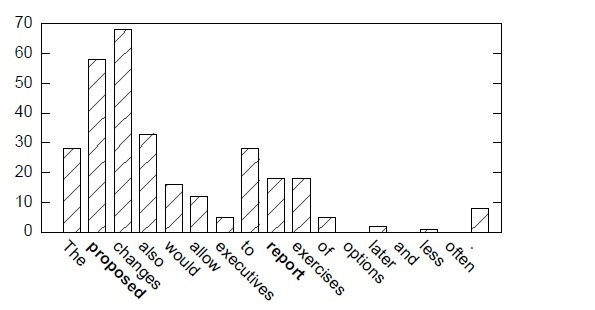
\includegraphics[scale=1.0]{C:/Users/Wei/Desktop/01.jpg}
\end{center}
2. classification   : Divided into four categories by word count.\\


a. Word Count $>$ 15 

b.15 $>$ Word Count $>$ 10

c. 10 $>$ Word Count $>$5 

d. 5 $>$Word Count

\begin{center}
	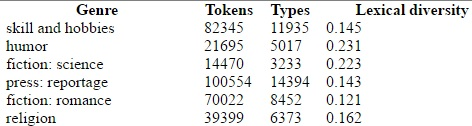
\includegraphics[scale=1.5]{C:/Users/Wei/Desktop/02.jpg}
\end{center}
3. search       : Search Word repetition rate in the article.\\
4. statistics     : count the repetition rate of words in the article.\\
5. sort         : Show the  number of occurrences of most rankings in every categorie.\\



\section*{Reference}
\label{sec:refe}

[1].Ralph Weiscbedel,Chairperson BBN Systems and Technologies Corporation Jaime Carbonell Carnegie-Mellon University Barbara Grosz Harvard University Wendy Lehnert University of Massachusetts, Amherst Mitchell Marcus University of Pennsylvania Raymond Perrault SRI International Robert Wilensky University of California, Berkeley   
\\\
[2].Ronan Collobert ,JasonWeston ,L�eon Bottou,Michael Karlen, Koray Kavukcuoglu, Pavel Kuksa, NEC Laboratories America4 Independence Way Princeton, NJ 08540





\end{document}      % End of the document
